\section{Proposition} \label{chapter4:proposition}

This thesis proposes a platform allowing a seamless shift of focus to follow the development of a web application from the productivity required in the early beginning until the efficiency required during maturation.
The proposed platform allows to develop applications targeting an event-driven platform allowing productivity, and transforms them so as to execute them on a pipeline architecture allowing efficiency.
% It is based on the transformation of an event-driven program to target a pipeline architecture.

% The event-driven platform is embodied by Javascript for the implementation of this thesis.
\textit{Node.js} is an efficient event-driven execution model to implement a web application.
Javascript features higher-order programming, dynamic typing and a global memory abstraction.
Because of these features, it is very productive.
% It makes Javascript a language of choice to develop web applications.
However, the efficiency of this execution model is limited by the sequentiality of execution required to preserve exclusivity of memory accesses.

On the other hand, the pipeline execution model doesn't present the same limitation.
It enforces memory isolation between stages allowing the parallel execution required for efficiency.
But this isolation limits the productivity of this execution model.

The difference in the memory abstractions between the two execution models is illustrated in figure \ref{fig:difference}.

% \subsection{Equivalence}

\begin{figure}[h!]
\begin{center}
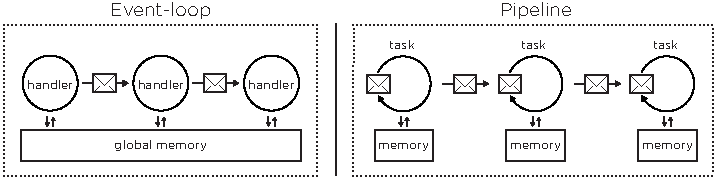
\includegraphics[width=0.9\textwidth]{../resources/models-difference.pdf}
\end{center}
\caption{Differences of memory abstraction}
\label{fig:difference}
\end{figure}


% The difference of memory model between the two execution model is illustrated in figure \ref{fig:mem-equivalence}.
Despite this difference, these two execution models present interesting similarities.
They both organize the execution as a sequence of tasks causaly scheduled. %, as illustrated in figure \ref{fig:run-equivalence}.

This thesis proposes an equivalence between the event-driven execution model and the pipeline execution model.
It distributes the global memory of the former into memory isolated stages of the latter.
% with message passing.
% As explained below, the concurrency model of the event-loop execution model, and the parallel approach of the pipeline execution model are very similar.
It transforms an event-driven application to run on a pipeline architecture.

\subsection{Continuous Development}

%It proposes this equivalence as a solution to allow the same platform to propose a continuity of compromises between productivity and efficiency.
This transformation allows a continuity of compromises between productivity and efficiency to continuously follow the shift of focus during development.
Developers keep two organizations of the implementation of an application. %, allowing them to start with productivity, and seamlessly abandon it for efficiency as the project matures.
The productive organization is based on the event-driven execution model.
It helps to maintain the application.
The efficient organization is the transformed application targeting the pipeline execution model.

At first, the focus remains on the productivity of development rather than the efficiency of execution.
The development begins with the event-driven model to take advantage of the productivity of the global memory abstraction.
% and the asynchronous control flow of the event-driven execution model.
The execution resulting from the transformation is as efficient as the original event-driven execution model.

During the maturation of the application, the focus continuously shift towards efficiency.
The transformation distribute the global memory into isolated stages as much as possible.
It allows developer to identify the dependencies in this global memory avoiding the distribution.
They can identify these dependencies, and arrange the implementation accordingly to allow parallelism.
It helps developers to enforce efficiency through continuous iteration, instead of disruptive shifts of technology.

% The next paragraphs introduce this equivalence.


\begin{figure}[h!]
\begin{center}
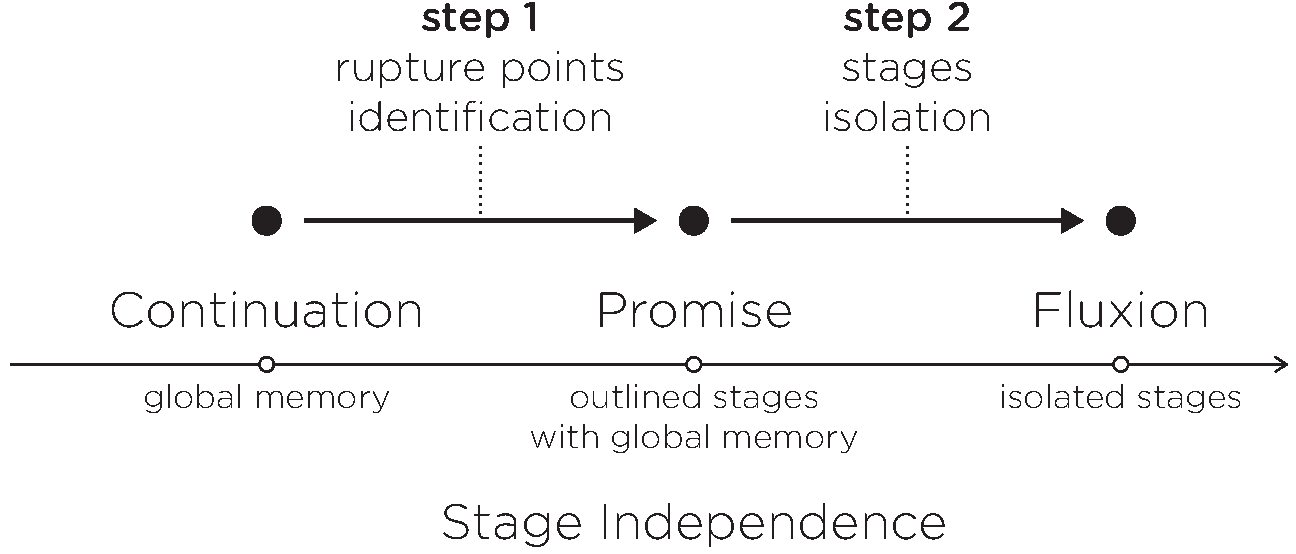
\includegraphics[width=0.7\textwidth]{../resources/roadmap.pdf}
\end{center}
\caption{Roadmap}
\label{fig:roadmap}
\end{figure}

\subsection{Equivalence} \label{chapter4:equivalence}

% The goal of this thesis is not to propose a new high-level language but to automate the architectural shift.
The next paragraphs introduces the equivalence between the the event-driven execution model and the pipeline execution model.
The equivalence is broken down in two steps, as illustrated in figure \ref{fig:roadmap}.
The first step identifies the rupture points in the control flow separating the stages of the pipeline.
The second step enforces isolation of memory between these stages, and replaces synchronization with message passing to preserve the invariance.
% invariance through message passing.

\subsubsection{Rupture Point}

\begin{wrapfigure}{r}{0.33\textwidth}
  \vspace{-10pt}
  \begin{center}
    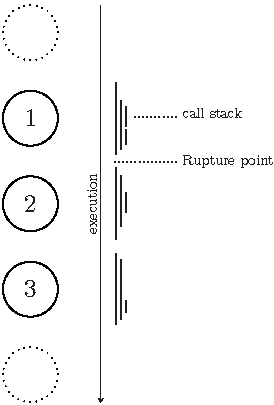
\includegraphics[height=0.4\textwidth]{../resources/rupture-point.pdf}
    \caption{Rupture point}
    \label{fig:rupture-point}
  \end{center}
  \vspace{-10pt}
\end{wrapfigure}

% The pipeline architecture enforces the memory isolation between stages.
In the pipeline architecutre, each stage has its own thread of execution independent from the others.
Whereas the handlers in the event-driven execution model are executed sequentially.
% the execution flow jumps from one concurrent handler to the other to execute them sequentialy.
%  because of the continuation passing style and the common memory store.
% The message passing linking the callbacks is transparently handled by the event-loop.
Despite this difference, the execution of a handler is as independent as the execution of a stage of a pipeline.
The call stacks of two handlers are isolated, as illsutrated in figure \ref{fig:rupture-point}.
Indeed, a handler holds the execution until all synchronous function calls terminates.
The asynchronous function call - the callee - between the caller and its continuation represents a rupture between the two call stacks.
And the call stack of the continuation is independent from the call stack of the caller and the callee.
This asynchronous callee represents a rupture point between two handlers.
It is equivalent to a data stream between two stages in the pipeline architecture.
It sends a message between the callee and the continuation.


% Both the pipeline architecture and the event-loop present these rupture points.
The detection of rupture points allows to map a pipeline architecture onto the implementation following the event-loop model.
% To allow the transformation from one to the other,
The proposed platform detects rupture points defining stages. %, and distributes the global memory into them.
This detection is fully addressed in the next chapter, in sections \ref{chapter5:due:compiler} and \ref{chapter5:flx:compiler}.
It presents the extraction of a pipeline of concurent tasks from a Javascript application.
% Such pipeline is similar to the one exposed by Promises.
% The chapter proposes a simpler alternative to the latter called Dues.
However, these stages still require a global memory.
They can't be executed in parallel.

\subsubsection{Invariance}

% This transformation is important on two points.
% The conservation of the invariance.
% The equivalence between the coordinations.

A global memory requires the sequential execution of handlers which implies the total scheduling with a queue, as illustrated in figure \ref{fig:total-scheduling}.
Whereas message passing only requires causal scheduling of handlers which allows parallelism.
Yet, the causal scheduling of tasks is sufficient to assure the correctness of the execution.
% The sequential execution is imposed by the global memory, not by the causality between handlers.
If the handlers didn't rely on the global memory, they could be executed in parallel, as long as their causalities are respected, as illustrated in figure \ref{fig:causal-scheduling}.

\begin{figure}[h!]
  \begin{minipage}[t]{0.20\textwidth}
    \centering
    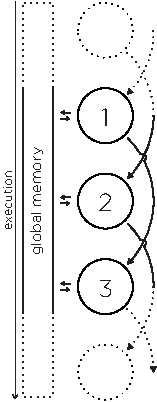
\includegraphics[page=1, height=2\linewidth]{../resources/invariance.pdf}
    \vfill
    \caption{Total scheduling}
    \label{fig:total-scheduling}
  \end{minipage}
  \hfill
  \vrule
  \hfill
  \begin{minipage}[t]{0.20\textwidth}
    \centering
    \includegraphics[page=2, height=2\linewidth]{../resources/invariance.pdf}
    \vfill
    \caption{Causal scheduling}
    \label{fig:causal-scheduling}
  \end{minipage}
  \hfill
  \vrule
  \hfill
  \begin{minipage}[t]{0.20\textwidth}
    \centering
    \includegraphics[page=3, height=2\linewidth]{../resources/invariance.pdf}
    \vfill
    \caption{Message passing memory update}
    \label{fig:memory-update}
  \end{minipage}
  \hfill
  \vrule
  \hfill
  \begin{minipage}[t]{0.20\textwidth}
    \centering
    \includegraphics[page=4, height=2\linewidth]{../resources/invariance.pdf}
    \vfill
    \caption{Sequential execution}
    \label{fig:sequential-execution}
  \end{minipage}
\end{figure}

If two handlers causally related rely on the same memory region, the global memory can be replaced by sending the updated memory by message.
As illustrated in figure \ref{fig:memory-update}, each handler has access only to its own memory.
The upstream handler communicate the memory update to the downstream handler.
However, if the downstream handler modifies this memory, it is not possible to distribute the memory.

If two handlers not causally related rely on the same memory region, they can access it in any order.
They need to be scheduled sequentially to maintain the exclusivity of access, as illustrated in figure \ref{fig:sequential-execution}.
The distribution of the global memory is fully addressed in section \ref{chapter5:flx:isolation}.

By distributing the global memory following these rules, the sequential scheduling can be loosen to causal scheduling to some extent, while preserving correctness.
% The global memory on which rely handlers is distributed and replaced with message passing.
This distribution only depends on the memory dependencies between handlers.
Developers can continuously iterate on implementation to loosen the depenencies between handlers to improve efficiency.





% As seen in the previous section, a sequential execution of handlers is interleaved by rupture points.




% Therefore, in the correctness of the execution, the ordering allowed by the global memory can be mapped to an equivalent message passing ordering.
% And it is possible to transform the global memory coordination into message passing.
% Given that the tasks are independent and communicate by messages.

% This result was used by Lamport to prove the correctness of distributed systems.
% Yet, to preserve the correctness as expressed by the developer, it is important to preserve the invariance provided by the global memory.
% The global memory needs to be distributed into each of the stages of the pipeline, so that each stage have an exclusive access to its memory.

% Moreover to assure the missing coordinations assured by the shared memory between the stages, the stages need to provide an equivalent coordination with message passing.





\subsubsection{Transformation}

Figures \ref{fig:run-equivalence} and \ref{fig:mem-equivalence} illustrate the two steps of the transformation in the context of the execution models.
Figure \ref{fig:run-equivalence} shows the identification of each handler from the event-driven execution model into a stage of the pipeline execution model.
Figure \ref{fig:mem-equivalence} shows the distribution of the global memory of the event-driven execution model into the different stages of the pipeline execution model.

The next section presents these two execution models and focus on the important details for this transformation.


\begin{figure}[h!]
  \begin{minipage}[t]{0.45\textwidth}
    \centering
    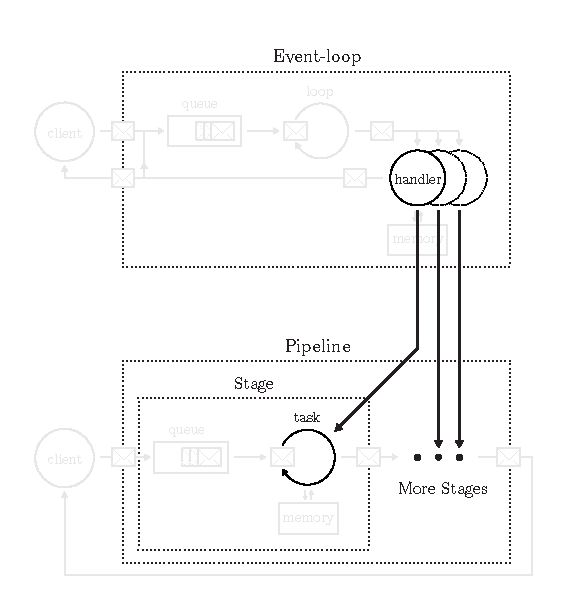
\includegraphics[width=\linewidth]{../resources/run-equivalence.pdf}
    \caption{Equivalence between handlers and tasks}
    \label{fig:run-equivalence}
  \end{minipage}
  \hfill
  \vrule
  \hfill
  \begin{minipage}[t]{0.45\textwidth}
    \centering
    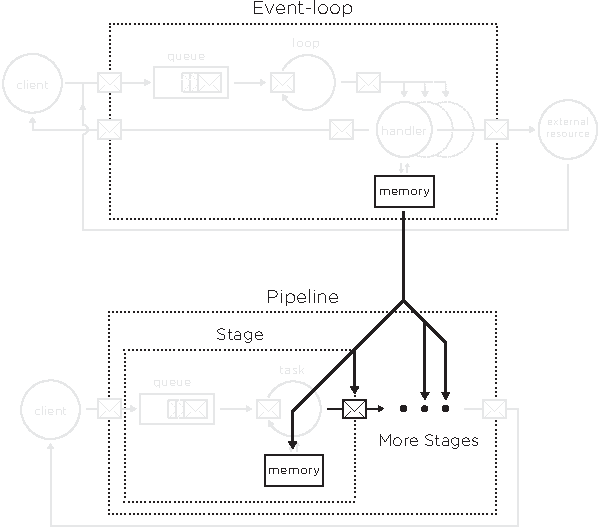
\includegraphics[width=\linewidth]{../resources/mem-equivalence.pdf}
    \caption{Distribution of the global memory abstraction with message passing}
    \label{fig:mem-equivalence}
  \end{minipage}
\end{figure}



% The invariance holds for the whole memory during the execution of each callback.
% As I explained in the previous section, this invariance is required to allow the concurrent execution of the different tasks.
% On the other hand, the invariance is explicit in the pipeline architecture, as all the stages have isolated memories.
% The coordination between these isolated process is made explicit by the developer through message passing.

% I argue that the state coordination between the callbacks requireing a global memory could be replaced by the message passing coordination used manually in the pipeline architecture.
% I argue that not all applications need concurrent access on the state, and therefore, need a shared memory.
% % Specifically, I argue that each state region remains roughly local to a stage during its modification.
% \nt{TODO review that, I don't know how to formulate these paragraphs. Identify the state and the data in the global memory.}

% \subsubsection{Transformation}

% This equivalence should allow the transformation of an event loop into several parallel processes communicating by messages.
% In this thesis, I study the static transformation of a program, but the equivalence should also hold for a dynamic transformation.
% I present the analyzis tools I developed to identify the state and the data from the global memory.